\documentclass[letterpaper,11pt]{article}
\usepackage{jheppub}
\usepackage{tikz}
\usepackage{float}
\usetikzlibrary{decorations.pathreplacing}
\usetikzlibrary{shapes.misc, positioning}
\setlength\parindent{20pt}



\definecolor{iocolor}{RGB}{169,205,236}
\definecolor{hlvcolor}{RGB}{224,235,245}
\definecolor{hscolor}{RGB}{166,166,166}
\definecolor{layercolor}{RGB}{218,218,218}
\definecolor{featcolor}{RGB}{202,203,229}
\definecolor{grucolor}{RGB}{222, 236, 239}

%\definecolor{hlvlinecolor}{RGB}{12, 178, 236}
%\definecolor{featurelinecolor}{RGB}{100, 159, 206}
\definecolor{hlvlinecolor}{RGB}{0, 148, 197}
\definecolor{featurelinecolor}{RGB}{0, 43, 152}
\definecolor{hslinecolor}{RGB}{85, 85, 85}



\begin{document}

%%%%%%%%%%%%%%%%%%%%%%
\section*{Anomalous Jet Identification via Variational Recurrent Neural Network}
Authors: Alan Kahn, Julia Gonski, In\^{e}s Ochoa*, Daniel Williams, Gustaaf Brooijmans \\ \textit{Nevis Laboratories, Columbia University, 136 S Broadway, Irvington NY}\\
\textit{*Laboratory of Instrumentation and Experimental Particle Physics, Lisbon, Portugal}\\


%\noindent \textit{Please do not write an introduction to anomaly detection - we will have one introduction at the beginning.  Furthermore, please give your method a concise name - it is fine to say \textbf{Concise Name: Longer Name that is More Specific.}  The length limit is five pages of text (not included references), with fewer pages preferred, and at most one additional page of figures if needed.}

\subsection{Method}
\label{sec:method}

%please introduce the motivation for your method (not anomaly detection in general), how it works, and how you have implemented it. Please include details about how you trained your algorithms and how your picked your hyperparameters.

\hspace{\parindent}The method described here employs a Variational Recurrent Neural Network (VRNN) to perform jet-level anomaly detection by modeling jets as a sequence of constituents. A VRNN is a sequence-modeling architecture which replaces the standard encoder-decoder architecture of a Recurrent Neural Network with a Variational Autoencoder (VAE)~\cite{chung2016recurrent}. 
This allows the VRNN to perform both sequence modeling in addition to variational inference, which has been shown to be a very powerful tool for anomaly detection~\cite{An2015VariationalAB}.
A sequence-modeling architecture is well-motivated as it is capable of accommodating variable-length inputs, such as lists of constituent four-vectors in a jet, while suppressing the ability of the model to learn correlations with the jet's constituent multiplicity.
By contrast, fixed-length architectures such as VAEs rely on a loss function that is computed between the input layer and the reconstructed output layer. As a result, zero-padded inputs directly affect the value of the loss function, leading to correlations that are difficult to remove when using inputs that are naturally variable in length, but forced to work in a fixed-length framework. 

Figure \ref{fig:VRNN} shows a diagram of one VRNN cell. The VAE portion of the architecture is displayed on the top row of layers in the diagram, where a constituent's four-momentum components are input as a vector $x(t)$, which is encoded into a multivariate Gaussian distribution in the latent space $z$, and then decoded to produce a reconstruction of the same input constituent's components $y(t)$. The variable $t$ refers to the \textit{time-step}, which advances as the sequence is processed, and can be interpreted as the constituent number currently being processed by the model. 


Inputs to the VRNN consist of sequences of jet four-vector constituent components $p_{T}$, $\eta$, and $\phi$, where constituents are assumed to be massless.
Jets are reconstructed using the anti-$k_t$ algorithm with a radius parameter of 1.0~\cite{Cacciari_2008}.
Before training, a pre-processing method is applied which boosts each jet to the same reference mass, energy, and orientation in $\eta-\phi$ space, such that all input jets differ only by their substructure.
In addition, our pre-processing method includes a choice of \textit{sequence ordering}, in which the constituent sequence input into the model is sorted by $k_{t}$-distance instead of by the typical constituent $p_{T}$. 
In more detail, the $n^{th}$ constituent in the list, $c_{n}$, is determined to be the constituent with the highest $k_{t}$-distance relative to the previous constituent, with the first constituent in the list being the highest $p_{T}$ constituent. 

\begin{equation}
c_{n} = max(p_{Tn}\Delta R_{n, n-1})
\end{equation}

This ordering is chosen such that non-QCD-like substructure, characterized by two or more separate prongs of constituents within in the jet, is more easily characterized by the sequence. 
When compared to $p_{T}$-sorted constituent ordering, the $k_{t}$-sorted sequence consistently travels between each prong, making their existence readily apparent and easy to model. As a result, a significant boost in performance is observed.

The loss function for each constituent, $\mathcal{L}(t)$, is very similar to that of an ordinary VAE. 
It consists of a mean-squared-error (MSE) loss between input constituents and generated output constituents as a reconstruction loss, as well as a weighted KL-Divergence from the learned latent space prior to the encoded approximate posterior distribution. 
Since softer constituents contribute less to the overall classification of jet substructure, each KL-Divergence term, computed constituent-wise, is weighted by the constituent's $p_{T}$-fraction with respect to the jet's total $p_{T}$, averaged over all jets in the dataset to avoid correlations with constituent multiplicity. 
The weight coefficient of the KL-Divergence term is enforced as a hyperparameter, and has been optimized to a value of 0.1 in dedicated studies. 

\begin{equation}
\mathcal{L}(t)=MSE+0.1 \times \overline{p_T}(t)D_{KL}
\end{equation}

After a jet is fully processed by the VRNN, a total loss function is computed as the average of the individual constituent losses over the jet: $\mathcal{L} = \frac{\Sigma \mathcal{L}(t)}{N}$.

The architecture is built with 16 dimensional hidden layers, including the hidden state, with a two-dimensional latent space. All hyperparameters used are determined by a hyperparameter optimization scan. 

The model is trained on the leading and sub-leading jets of each event, where events are taken from the LHC Olympics datasets. 
After training, each jet in the dataset is assigned an \textit{Anomaly Score}, defined in Equation~\ref{eq:as}, where $D_{KL}$ is the KL-Divergence from the learned prior distribution to the encoded posterior distribution.

\begin{equation}
\label{eq:as}
\text{Anomaly Score} = 1 - e^{-\overline{D_{KL}}}
\end{equation}

Since the LHC Olympics challenge entails searching for a signal on the event-level instead of the jet-level, an overall \textit{Event Score} is determined by choosing the most anomalous score between the leading and sub-leading jets in an event. 
To ensure consistency between training scenarios, Event Scores are subject to a transformation in which the mean of the resulting distribution is set to a value of 0.5, and Event Scores closer to 1 correspond to more anomalous events. 


%VRNN Diagram
\begin{figure}
  \begin{center}
  
    %\def\layersep{2.5cm}
   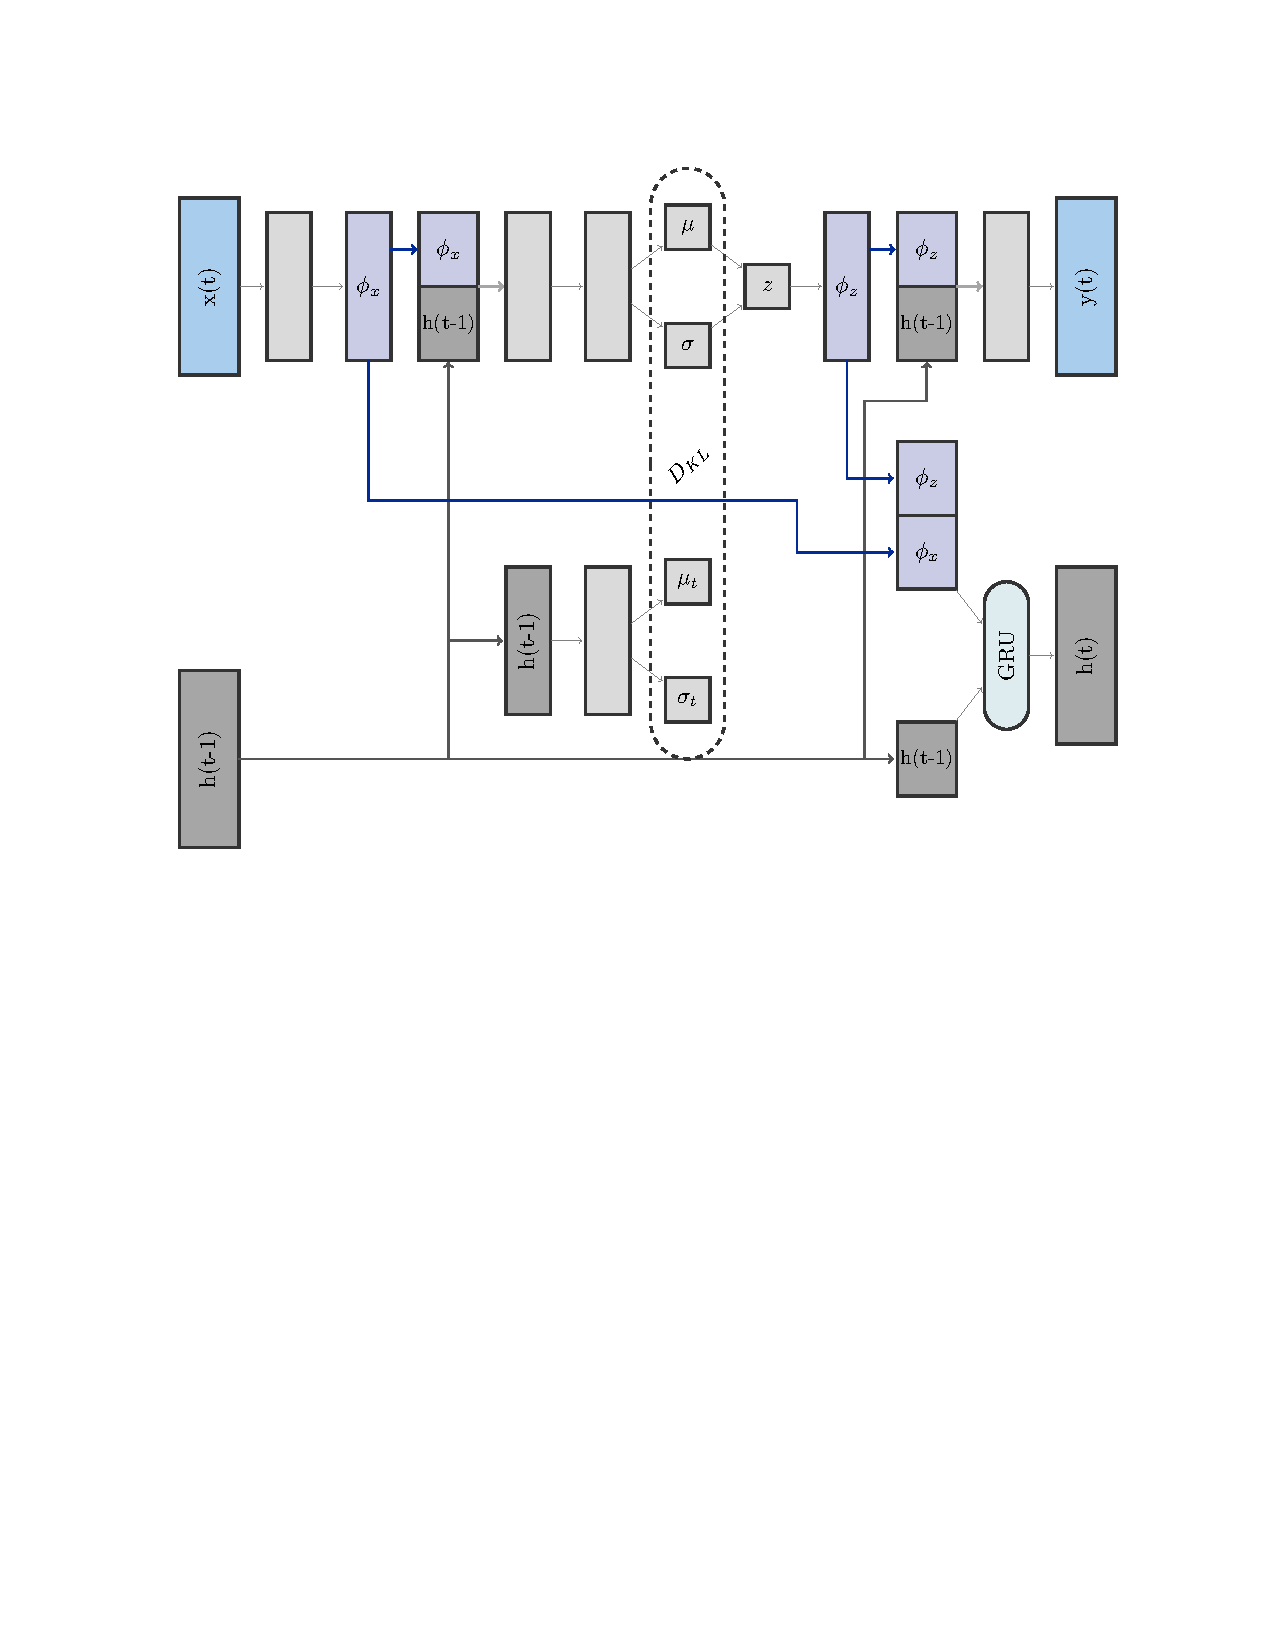
\includegraphics[width=0.8\textwidth]{imgs/VRNN_Diagram.pdf}
  
  \end{center}
  \caption{A Variational Recurrent Neural Network cell. The $x(t)$ and $y(t)$ layers represent respectively the input constituent and reconstructed constituents' four-momentum components $p_{T}$, $\eta$, and $\phi$. The $\phi_{x}$ and $\phi_{z}$ layers are \textit{feature-extracting layers} which encode a representation of the features in the input layer $x(t)$ and latent space $z$ respectively. $h(t-1)$ represents the current time-step's hidden state, which is updated each iteration via a transition function between $h(t-1)$, $\phi_{x}$, and $\phi_{z}$ carried out by a Gated Recurrent Unit (GRU). At each time-step, the prior distribution defined by $\mu_{t}$ and $\sigma_{t}$ is determined from the current hidden state}
  \label{fig:VRNN}
\end{figure}


%---------------------------------------------------------------------------------------------------------------------------------------------------------
%---------------------------------------------------------------------------------------------------------------------------------------------------------
\subsection{Results on LHC Olympics}
\label{sec:results}

%\noindent \textit{We welcome results on any of the black boxes (BBs) as well as the R\&D dataset.  Please try to minimize any discussion of non-LHCO results.  Figures should be referenced like this: Fig.~\ref{fig:fig1}.

\hspace{\parindent}The performance of the VRNN was first assessed with the LHC Olympics R\&D dataset, which includes a known signal of a beyond-the-Standard-Model W' boson with a mass of 3500GeV which decays to two hadronically decaying X and Y particles, each reconstructed by a R=1.0 jet.
This study was used as a validation of the method, with a goal of directly investigating the ability of the Event Score selection to reconstruct the W' mass. 
Therefore, no selections beyond those described in Section~\ref{sec:method} are applied.


The VRNN was trained over a contaminated dataset consisting of 895113 background events and 4498 signal events, corresponding to a signal contamination level of 0.5\%.
A selection on the Event Score is applied as the sole discriminator, and the invariant mass $m_{JJ}$ of the two jets is then scanned to assess the prominence of the W' mass peak.
In this validation analysis, the Event Score is required to exceed a value of 0.65. 
This value is chosen to significantly enrich the fraction of anomalous jet events over the background, while retaining enough statistics in the background to display its smoothly falling behavior.

Figure \ref{fig:m_JJ} shows the dijet invariant mass distributions before and after the Event Score selection, along with the local significance of the signal computed in each bin using the {\sc BinomialExpZ} function from {\sc RooStats} with a relative background uncertainty of 15\%~\cite{moneta2011roostats}.
Applying this selection dramatically increases the significance of the excess from $0.18\sigma$ to $2.2\sigma$ without significantly sculpting the shape of the background.


\begin{figure}[h!]
	\begin{center}
		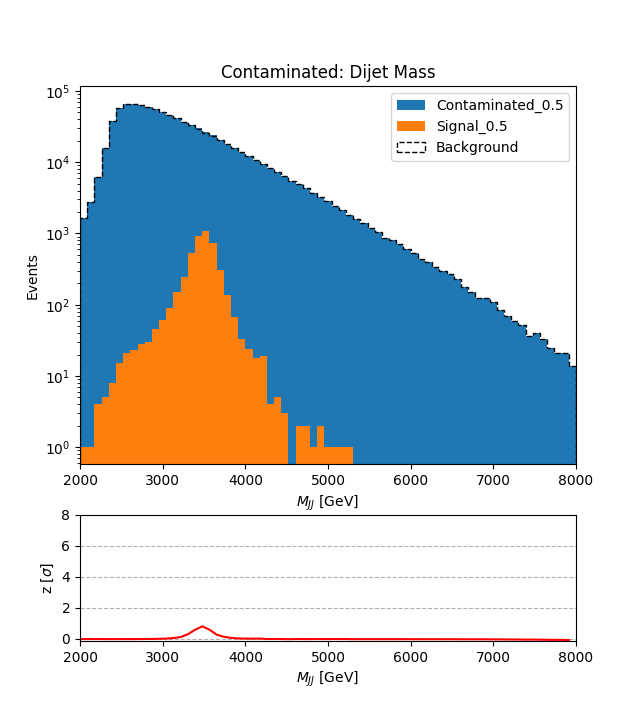
\includegraphics[width=0.47\textwidth]{imgs/2Prong_Contaminated_0p5_JJ_Mass_Multi.png}
		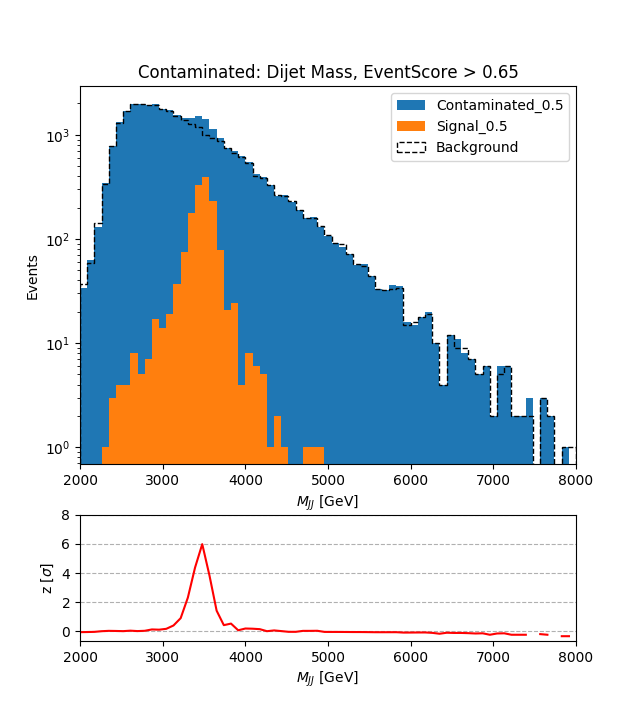
\includegraphics[width=0.47\textwidth]{imgs/2Prong_Contaminated_0p5_JJ_Mass_EventScore0p65_Multi.png}
	\end{center}
	\caption{Dijet invariant mass distributions before (left) and after (right) a selection on the Event Score, with a two-prong W' signal contamination of 0.5\%.}
	\label{fig:m_JJ}
\end{figure}

Once the method was validated in the R\&D dataset, it was applied to Black Box 1, with a re-optimized tighter selection on the Event Score of 0.75, as well as a requirement on the pseudorapidity of the leading and sub-leading jets to be less than 0.75, to ensure that central, high momentum transfer events are considered. Figure {\ref{fig:bb1}} shows the dijet invariant mass for both the Black Box 1 and Background datasets. The Event Score selection reveals an enhancement in $m_{JJ}$ just below 4000 GeV. This is consistent with the Black Box 1 signal, which is a new Z' boson with a mass of 3800 GeV decaying to two new particles, each decaying hadronically.

\begin{figure}[h!]
	\begin{center}
		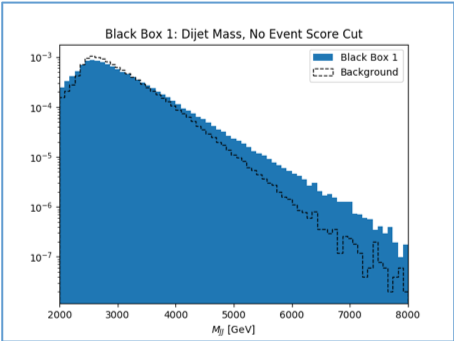
\includegraphics[width=0.47\textwidth]{imgs/BB1.png}
		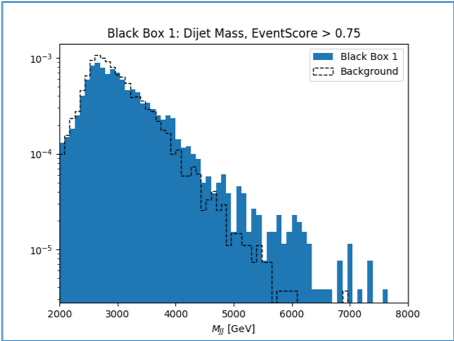
\includegraphics[width=0.47\textwidth]{imgs/BB1_Cut.png}
	\end{center}
	\caption{Dijet invariant mass distributions before (left) and after (right) a selection on the Event Score from the Black Box 1 dataset. The signal present is a Z' boson with a mass of 3800 GeV.}
	\label{fig:bb1}
\end{figure}

The same method applied to Black Box 2, shown in Figure \ref{fig:bb2}, results in no significant excesses in the invariant mass distribution. Additionally, the effect of the Event Score selection on the $m_{JJ}$ shapes is similar between the Black Box 2 and Background datasets. Black Box 2 does not contain any beyond-the-Standard-Model events, and therefore these results are consistent with a QCD-only sample. It is important to note that the model was trained independently on each dataset, and the resulting Event Scores are from entirely unique sets of network weights.

\begin{figure}[h!]
	\begin{center}
		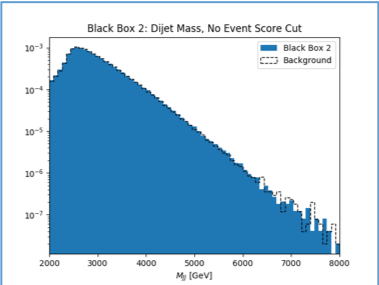
\includegraphics[width=0.47\textwidth]{imgs/BB2.png}
		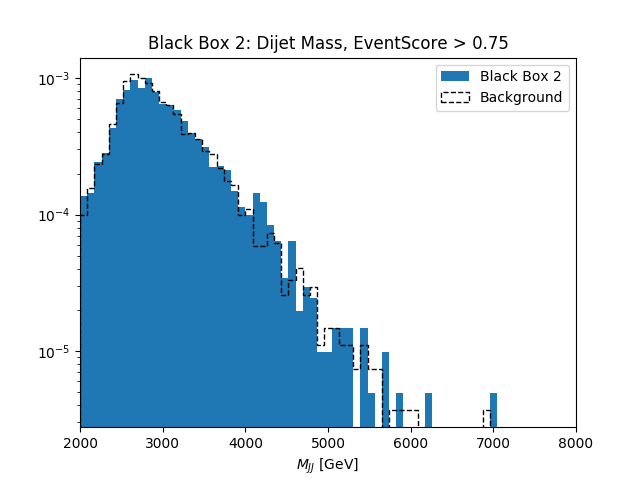
\includegraphics[width=0.47\textwidth]{imgs/BB2_Cut.png}
	\end{center}
	\caption{Dijet invariant mass distributions before (left) and after (right) a selection on the Event Score from the Black Box 2 dataset. No signal is present, and the dataset shown consists entirely of multijet background events.}
	\label{fig:bb2}
\end{figure}

Figure \ref{fig:bb3} shows results for Black Box 3. The signal in Black Box 3 consists of a new 4200 GeV particle, with varied final states beyond the two-prong large-$R$ jets described earlier. As the model described here is specifically sensitive to substructure within a large-$R$ jet, it is insensitive to the signal present in this Black Box. 

\begin{figure}[H]
	\begin{center}
		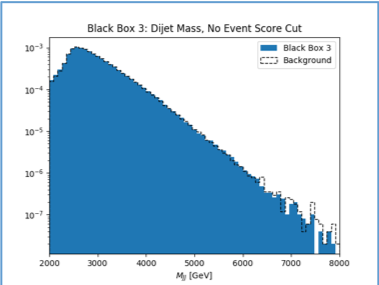
\includegraphics[width=0.47\textwidth]{imgs/BB3.png}
		\includegraphics[width=0.47\textwidth]{imgs/BB3_Cut.png}
	\end{center}
	\caption{Dijet invariant mass distributions before (left) and after (right) a selection on the Event Score from the Black Box 3 dataset. The signal present is a new boson with a mass of 4200 GeV.}
	\label{fig:bb3}
\end{figure}


\subsection{Lessons Learned}
\label{sec:lessons}

%\noindent \textit{Please say anything that you learned from the experience in general, what you learned specifically from the results, what you improved after you learned about BB1, what you would change in the future, etc.}

\hspace{\parindent}This challenge presented a highly useful avenue for development of our model. 
Results from the R\&D and Black Box dataset analyses indicate that the VRNN is capable of identifying anomalous objects within a contaminated dataset as long as they can be characterized by sequential data. 
We learned that the pre-processing method is hugely influential on the performance of the model, in particular the choice of $k_{t}$-ordered sequencing. 
We feel that this is a generalizable conclusion from our study which can be applied to the understanding and use of jet substructure in future analyses.

Given these lessons, there are a variety of future opportunities with this application of the VRNN architecture to jet-level anomaly detection. 
Since the VRNN takes constituent information as input and learns jet substructure without explicit reliance on high level variables, it is expected to have less correlation with jet mass than standard substructure variables such as N-subjettiness. Further characterization of this point could reveal a key advantage in using such an approach in an analysis context.
While we limited our scope in this study to be entirely unsupervised with no signal or background model information, the RNN and VAE elements of the VRNN give potential for accommodating more supervised training scenarios. 
Furthermore, a number of advancements to the architecture, such as a dedicated adversarial mass de-correlation network, or an additional input layer representing high-level features, are worthwhile avenues of exploration to enhance performance while minimizing unwanted correlations. 


%%%%%%%%%%%%%%%%%%%%%%%%
\acknowledgments

This material is based upon work supported by the National Science Foundation under Grant No. PHY-2013070.

%\vspace{10mm}

%\noindent \textit{For the references, please use names from Ref.~\cite{hepmllivingreview}.  If your paper is not there or is not updated, please submit a MR!}

\bibliographystyle{jhep}
%\bibliography{contribution}
\bibliography{HEPML,contribution}
\end{document}
